\documentclass{article}
\usepackage{iclr2024_conference,times}
\input{math_commands.tex}

\usepackage{hyperref}
\usepackage{url}
\usepackage{booktabs}
\usepackage{amsmath}
\usepackage{graphicx}
\usepackage{subcaption}
\usepackage{tikz}
\usetikzlibrary{arrows.meta,positioning,calc}
\usepackage{float}
\graphicspath{{figures/}}

\title{Behavioral Deduplication and Diversity-Guided\\
Selection for Sample-Efficient FunSearch}

\author{CHEN Sijie (59872908) \& BIAN Wenbo (59872472) \\
Department of Computer Science, City University of Hong Kong \\
\texttt{sijiechan2-c@my.cityu.edu.hk}, \texttt{wbian9-c@my.cityu.edu.hk}}

\iclrfinalcopy
\begin{document}
\maketitle

\begin{abstract}
We propose \textbf{behavioral-fingerprint deduplication} for FunSearch, an LLM-driven
evolutionary program search framework. LLM proposers repeatedly produce functionally
equivalent heuristics: on an unmodified run we observe $45\%$ of proposals scoring
identically to an ancestor---a conservative proxy for behavioural redundancy that
wastes costly API calls and sandbox evaluations.
Our method executes each candidate on ten lightweight probing instances, hashes the
resulting $375$-dimensional decision sequence, and rejects exact matches before full
evaluation; we further integrate filter-level diversity and ReEvo reflective evolution
\citep{ye2024reevo} into the same pipeline.
On OR3 online bin packing under a $150$-sample budget, deduplication alone reduces
\emph{samples-to-best} by $38\%$ ($146\to 90$) without degrading the best score. An
offline \textbf{Behavioural Coverage Rate (BCR)} analysis ($n{=}1$ per condition,
exploratory) suggests that deduplication alone may reach broader behavioural coverage
than deduplication combined with filter-level diversity---a hypothesis flagged for
multi-seed follow-up. Adding ReEvo on top of deduplication and filter-level diversity
yields the lowest-variance condition in our runs (mean $-209.66$, std $0.59$, $n{=}4$),
consistent with the landscape-smoothing mechanism reported by \citet{ye2024reevo}.%
\footnote{Reproducibility: \url{https://colab.research.google.com/github/jaycee6666/efficient-funsearch/blob/main/notebooks/efficient_funsearch_colab.ipynb}.}
\end{abstract}

\section{Introduction}
\label{sec:intro}

FunSearch \citep{romera2023mathematical} evolves programs by iterating an LLM proposer
against an evaluator: each round, the LLM drafts a new heuristic given recent
high-scoring ancestors, and a sandbox measures the candidate's score. The paradigm has
recently been scaled up to industrial settings --- AlphaEvolve \citep{alphaevolve2025}
reports substantial improvements on Google Borg datacenter scheduling using this same
LLM-evolve loop --- and online bin packing has emerged as one of its canonical
benchmarks \citep{sim2025bin,liu2024eoh}. Under limited API budgets, however, the
\emph{sample efficiency} of the proposer becomes the central differentiator
\citep{ye2024reevo}: the question is not whether a reasonable heuristic can be found,
but how many LLM calls it takes.

Our preliminary baseline exposes a concrete waste source. Running unmodified FunSearch
on the OR3 instance set for $53$ samples, $45\%$ of all programs produced scores
\emph{identical} to programs already in the archive---a conservative proxy for
behavioural redundancy (same score need not imply same per-item decision sequence,
but the converse holds) that syntactic hashing does not catch, and which the
$375$-dimensional fingerprint introduced in \S\ref{sec:method} verifies directly. This matches
the open direction identified by \citet{vanstein2025llm}, who argue that niching and
portfolio-style behavioural analysis are under-explored in LLM-driven
meta-heuristics. Existing FunSearch variants do not deduplicate at the behavioural
level and do not explicitly constrain diversity of accepted programs.

This paper makes three contributions. \textbf{(Main)} A three-level
\emph{behavioural-fingerprint funnel} (AST-hash $\to$ probing-fingerprint match $\to$
a disabled cosine layer), inspired by ReEvo's F-value deduplication
\citep{ye2024reevo} but lifted to the behaviour level; on OR3 under a $150$-sample
budget it reduces \emph{samples-to-best} by $38\%$ without degrading best score.
\textbf{(Extension)} We integrate filter-level diversity and ReEvo reflective
evolution on top of deduplication inside the same pipeline and analyse their
stacked behaviour; reflection-only is not separately ablated (\S\ref{sec:lim}~\#6),
and the complete $\mathrm{Score}(c)=\mathrm{Perf}(c)+\beta\cdot\mathrm{Div}(c)$
cluster scoring is future work. \textbf{(Tool)} We introduce an offline \textbf{Behavioural Coverage Rate} (BCR)
metric inspired by MAP-Elites \citep{mouret2015illuminating}; on an exploratory
pair of runs ($n{=}1$ per condition) it suggests that deduplication alone may
reach full behavioural coverage faster than deduplication combined with
filter-level diversity, consistent with the view that at the behaviour level
\emph{removing redundancy} and \emph{promoting novelty} may not be simply additive
\citep{vanstein2025llm}.

\section{Method}
\label{sec:method}

\subsection{Pipeline Overview}
\label{sec:pipeline}

The original FunSearch pipeline alternates between an LLM sampler and a sandboxed
evaluator, with island-based selection maintaining diversity at the population level
\citep{romera2023mathematical}. Our enhanced pipeline inserts a deduplication funnel
\emph{before} the expensive sandbox, and optionally wires in filter-level diversity
and ReEvo reflection around the database (Figure~\ref{fig:pipeline}). Only programs
surviving all enabled dedup levels incur a full sandbox evaluation; accepted programs
additionally trigger a lightweight LLM reflection call whose output is stored and
replayed as prompt context in later rounds.

\begin{figure}[t]
\centering
\resizebox{0.96\linewidth}{!}{%
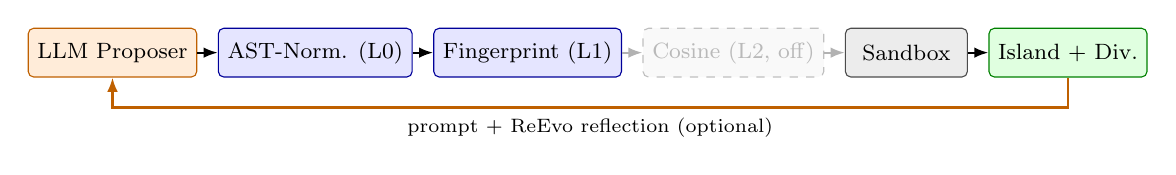
\begin{tikzpicture}[
  node distance=0.26cm and 0.26cm,
  box/.style={draw, rounded corners=2pt, minimum height=0.62cm,
              minimum width=1.55cm, align=center, font=\footnotesize},
  dedup/.style={box, fill=blue!10, draw=blue!60!black},
  disabled/.style={box, fill=gray!5, draw=gray!50, dashed, text=gray!55},
  sandbox/.style={box, fill=gray!15, draw=gray!60!black},
  archive/.style={box, fill=green!12, draw=green!50!black},
  llm/.style={box, fill=orange!15, draw=orange!75!black},
  arr/.style={-{Latex[length=1.8mm]}, thick},
  darr/.style={-{Latex[length=1.8mm]}, thick, dashed, gray!60},
  looparr/.style={-{Latex[length=1.8mm]}, thick, orange!75!black},
]
\node[llm] (llm) {LLM Proposer};
\node[dedup, right=of llm] (ast) {AST-Norm. (L0)};
\node[dedup, right=of ast] (fp) {Fingerprint (L1)};
\node[disabled, right=of fp] (l2) {Cosine (L2, off)};
\node[sandbox, right=of l2] (sb) {Sandbox};
\node[archive, right=of sb] (arch) {Island + Div.};

\draw[arr] (llm) -- (ast);
\draw[arr] (ast) -- (fp);
\draw[darr] (fp) -- (l2);
\draw[darr] (l2) -- (sb);
\draw[arr] (sb) -- (arch);

\coordinate (archdown) at ($(arch.south) + (0,-0.38)$);
\coordinate (llmdown)   at ($(llm.south)  + (0,-0.38)$);
\draw[looparr] (arch.south) -- (archdown) --
    node[midway, below, font=\scriptsize, text=black]
    {prompt + ReEvo reflection (optional)}
    (llmdown) -- (llm.south);
\end{tikzpicture}%
}
\caption{System pipeline. Candidates are normalised (L0) and fingerprinted
(L1) before sandbox evaluation; cosine (L2) is retained in code but disabled
at run time (Section~\ref{sec:fp}). Survivors enter an island archive with
filter-level diversity; archived programs feed the LLM via prompt
construction and, optionally, ReEvo reflection.}
\label{fig:pipeline}
\end{figure}

\subsection{Behavioral Fingerprint}
\label{sec:fp}

\textbf{Probing instances.} We hand-designed $10$ bin-packing probes spanning
uniform-medium, large-item, small-varied, bimodal, descending-spread, ascending-spread,
sawtooth, tight-pairs, wide-capacity, and an OR3-derived sample (Appendix~\ref{app:probes}).
Capacity is drawn from $\{100,150,200\}$ and items from $[20,140]$ to match the OR3
distribution; each probe contains $35$--$40$ items, for a total of $375$ decisions.

\textbf{Fingerprint definition.} For a candidate priority function $f$ and probe
$p_i$, we simulate the online first-fit-by-priority assignment: at each step the bin
with the highest $f(item,bins)$ is chosen (opening a new bin when needed). The
$k$-th decision is the index of the chosen bin. Concatenating the decisions across all
ten probes yields a deterministic $375$-dimensional integer tuple, the program's
\emph{behavioural fingerprint}.

\textbf{Three-level funnel.} Level~0 normalises the candidate source (variable
renaming, comment stripping) through an AST rewriter and hashes the result with
SHA-256. Level~1 hashes the fingerprint tuple and performs an $O(1)$ exact-match
lookup against an archive. On the proxy probe set, Level~1 matches are exact by
construction; at the \emph{fingerprint-match stage} this produces no threshold-based
false positive (we discuss the generalisation of this equivalence to out-of-distribution
inputs in \S\ref{sec:disc} Insight~2 and \S\ref{sec:lim}~\#4).
Level~2 was implemented as a cosine-similarity check with threshold $0.98$; a
calibration on $53$ baseline programs showed that $98.5\%$ of genuinely different
programs would be flagged duplicate, so it is disabled and kept only as a negative
result (\S\ref{sec:disc} Insight~2).

\textbf{Overhead.} Normalisation is $<1$\,ms, executing one probe $<3$\,ms, the
overall fingerprint $<50$\,ms, and the hash lookup negligible --- all dominated by
the $\sim 11$\,s sandbox evaluation they replace.

\subsection{Filter-Level Diversity}
\label{sec:div}

We use the term \emph{filter-level diversity} throughout to denote the following
variant: after a candidate passes the Level-1 fingerprint check, we additionally
discard it if its fingerprint's cosine similarity to \emph{any} recent island
representative exceeds a threshold. This biases the proposer toward behaviourally
under-represented regions without modifying the island's softmax cluster sampling
inside \texttt{programs\_database.py}. We emphasise that our experiments do not
evaluate the full cluster score
$\mathrm{Score}(c)=\mathrm{Perf}(c)+\beta\cdot\mathrm{Div}(c)$ with adaptive $\beta$
scheduling (listed as future work in \S\ref{sec:lim});\; all mentions of ``diversity''
in the remainder of this paper refer to this filter-level variant.

\subsection{ReEvo Reflective Evolution}
\label{sec:reevo}

Following \citet{ye2024reevo}, we add a per-accepted-program reflection step: after a
program is scored, the LLM is asked in $1$--$2$ sentences to describe the algorithmic
strategy the program uses and how it differs from a simple greedy approach. We keep
the top-$3$ highest-scoring reflections and inject them as comments into the next
prompt as ``strategy insights from top-performing programs'' (full prompt in
Appendix~\ref{app:reevo}). Context: ReEvo's landscape-smoothing analysis
\citep[Table~4]{ye2024reevo} reports a $4.5\times$ increase in correlation length and
$45.8\%$ objective improvement on related heuristic-design benchmarks, which provides
a plausible mechanism consistent with the variance reduction we observe
(\S\ref{sec:results}).

\subsection{Offline Behavioural Coverage Rate (BCR)}
\label{sec:bcr}

BCR is a post-hoc diagnostic that characterises how quickly a run visits distinct
behavioural regions. It is defined only for fingerprint-exporting conditions
(\emph{dedup}, \emph{dedup+div}); baseline bypasses the filter, and our ReEvo run
did not set \texttt{EXPORT\_FINGERPRINTS=1}. Given the union of fingerprints, we fit
a single $k$-means ($K{=}8$) once, then replay each condition's time series:
$\mathrm{BCR}(t)=|\{c(\mathbf{f}_s):s\le t\}|/K$. Offline fit-then-replay avoids
cluster-relabelling drift at this sample size. The coverage intuition follows
MAP-Elites \citep{mouret2015illuminating,alphaevolve2025}; we do not claim alignment
with van Stein et al.'s runtime-trajectory definition \citep{vanstein2025llm}.

\section{Experiments}
\label{sec:exp}

\subsection{Setup}
\label{sec:setup}

\textbf{Task.} Online bin packing (OBP) receives items $s_1, s_2, \dots$ one at a
time and must assign each to a bin irrevocably on arrival; the heuristic $h$ scores
every open bin and places the item in the highest-scoring feasible one (or opens a
new bin). The score reported in this paper is
$-\tfrac{1}{|\mathcal{D}|}\sum_{d\in\mathcal{D}} \mathrm{bins\_used}(h, d)$, i.e.,
the negated mean number of bins used over $|\mathcal{D}|{=}20$ OR3 files
(\texttt{u500\_00}--\texttt{u500\_19}, each $500$ items, capacity $150$); higher is
better. The L1 lower bound $\lceil\sum s_i/C\rceil$ averages to $-201.2$ on OR3, so
a score of $-209.66$ corresponds to $\sim 8.5$ bins above the theoretical minimum.
All experiments use OR3 for evaluation and Weibull-5k as auxiliary data, following
the FunSearch evaluation protocol \citep{romera2023mathematical}. The LLM
proposer is \texttt{gpt-5-nano} via the course API, with $10$ islands, $4$
samples-per-prompt, and a $30$\,s sandbox timeout. Each run is capped at $150$ LLM
samples --- well below the $20{,}000$-call budget --- to keep the comparison within
the ``low-sample regime'' studied by \citet{ye2024reevo}. We evaluate four
conditions: \textit{baseline} (unmodified FunSearch, $n{=}2$), \textit{dedup}
(fingerprint funnel only, $n{=}4$), \textit{dedup+div} (funnel plus filter-level
diversity, $n{=}4$), and \textit{reevo} (funnel + filter-level diversity + ReEvo
reflection stacked, $n{=}4$; reflection-only is not separately ablated---see
\S\ref{sec:lim}~\#6). Total API usage across all runs is $\sim 2{,}100$ calls.

\subsection{Main Results}
\label{sec:results}

\begin{figure}[t]
\centering
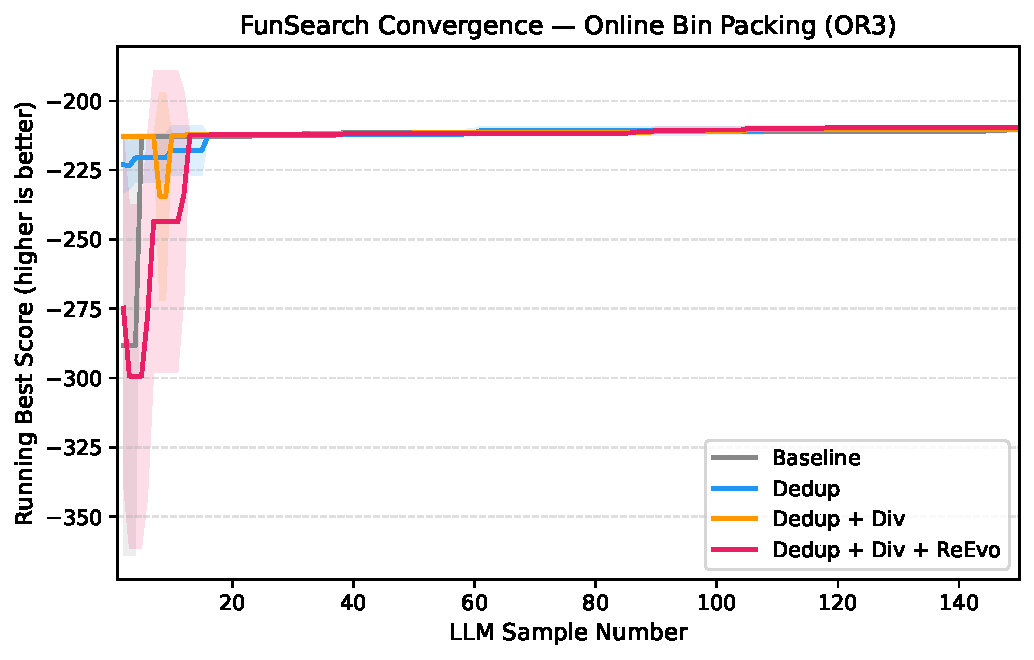
\includegraphics[width=0.65\linewidth]{convergence_150.pdf}
\caption{Best-score convergence versus sample number across the four conditions
(mean $\pm$ std band, $n{=}2$--$4$). All conditions land within $-210\pm 1$; the
ReEvo condition is the only one whose mean is below $-210$.}
\label{fig:conv}
\end{figure}

\begin{table}[t]
\centering\small
\caption{Main results at a $150$-sample budget. \emph{Samples-to-best} is the first
sample number at which a run attains its best score; \emph{Dup rate} is the fraction
of candidates rejected by the dedup filter (N/A for baseline, which bypasses the
filter).}
\label{tab:main}
\begin{tabular}{lcccc}
\toprule
Condition & $n$ & Best score (mean $\pm$ std) & Samples-to-best & Dup rate \\
\midrule
Baseline   & 2 & $-210.52 \pm 1.31$ & $146 \pm 2$  & N/A \\
Dedup      & 4 & $-210.04 \pm 1.00$ & $\mathbf{90 \pm 36}$ & $0.401 \pm 0.046$ \\
Dedup+Div  & 4 & $-210.20 \pm 0.68$ & $108 \pm 21$ & $0.342 \pm 0.067$ \\
\textbf{ReEvo} & 4 & $\mathbf{-209.66 \pm 0.59}$ & $101 \pm 16$ & $0.314 \pm 0.034$ \\
\bottomrule
\end{tabular}
\end{table}

Table~\ref{tab:main} and Figure~\ref{fig:conv} reveal four observations.

\textbf{(O1) Main contribution.} Baseline$\to$Dedup reduces samples-to-best from $146$
to $90$, a \textbf{$38.4\%$ reduction} in the number of LLM samples the proposer
consumes before the run's best program is discovered. The best score itself is
unchanged ($-210.52\to -210.04$).

\textbf{(O2) No observable performance degradation.} All four conditions have best
scores in $-210\pm 1$. At this budget and sample size ($n{=}2$--$4$) we observe no
measurable best-score cost from deduplication, filter-level diversity, or reflection
--- an observation consistent with (but, per \S\ref{sec:disc} Insight~2, not a direct
verification of) a low false-positive rate on the full input distribution.

\textbf{(O3) Full stack yields the lowest variance.} The \textit{reevo} condition
(dedup $+$ diversity $+$ reflection) is the only one whose mean is below $-210$
($-209.66 \pm 0.59$). This is qualitatively consistent with the landscape-smoothing
effect reported for reflection by \citet{ye2024reevo}, but because reflection is
stacked on top of dedup and filter-level diversity in these runs, we cannot
separately attribute the improvement to reflection; $n{=}4$ is also insufficient for
significance testing.

\textbf{(O4) Dup rates decrease as extra signals are added.} Among dedup-equipped
conditions, the rejection rate drops from $0.401$ (dedup) to $0.342$ (dedup+div) to
$0.314$ (reevo). Because the archive distribution and prompt context co-vary across
these conditions (stronger signals also change which programs survive into the
archive), we read this as a correlational observation rather than evidence that
diversity or reflection causally pushes the LLM toward new behaviours. (We do not
include baseline in this trend because it does not route candidates through the
dedup filter; the $45\%$ natural duplicate rate mentioned in \S\ref{sec:intro} is
computed independently on identical-score counts.)

\subsection{Behavioural Coverage Analysis}
\label{sec:bcr-exp}

\begin{figure}[t]
\centering
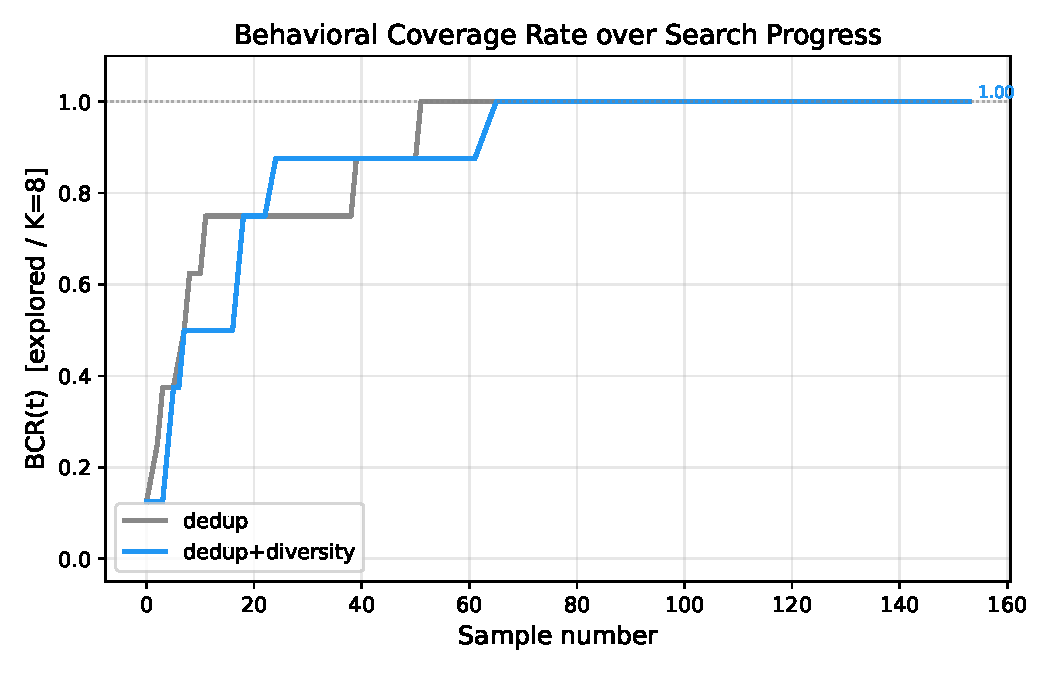
\includegraphics[width=0.65\linewidth]{bcr_curves.pdf}
\caption{Behavioural Coverage Rate over sample index (exploratory; $n{=}1$ per
condition). Dedup-only (blue) reaches full coverage (BCR$=1$) at sample $51$;
Dedup+Div (orange) reaches full coverage at sample $65$. Only these two conditions
export fingerprints in the current run set.}
\label{fig:bcr}
\end{figure}

Figure~\ref{fig:bcr} plots BCR$(t)$ for the two fingerprint-exporting conditions
($n{=}1$ each; this is exploratory rather than a mechanism claim):
Dedup-only reaches $\mathrm{BCR}=1.0$ at sample $51$, whereas Dedup+Div takes until
sample $65$. \textbf{Reverse-intuitive observation:} under this single pair of runs,
filter-level diversity appears to \emph{slow} cluster visitation. A plausible
reading is that once duplicates are filtered, retained samples are already diverse
by construction, so the extra diversity constraint concentrates exploration within
already-reached clusters rather than reaching new ones; confirming this would
require multi-seed replication at the same $n$ used for the main table
\citep{vanstein2025llm}.

\subsection{Fingerprint Space Visualisation}
\label{sec:tsne-exp}

\begin{figure}[t]
\centering
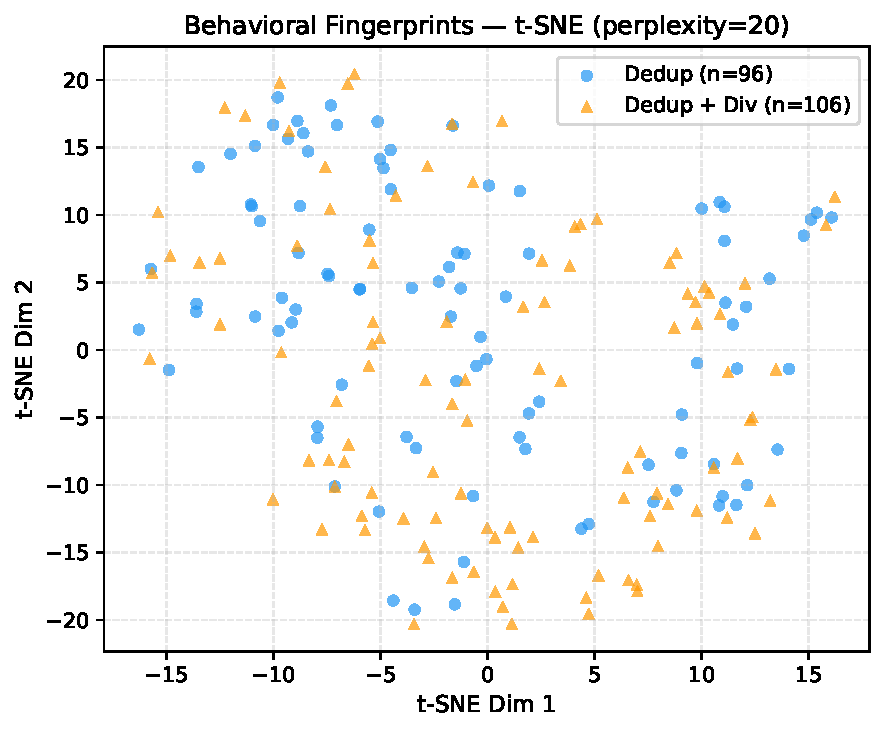
\includegraphics[width=0.62\linewidth]{tsne_fingerprints.pdf}
\caption{t-SNE ($perplexity{=}20$) of $\sim 200$ fingerprint vectors (each $375$-dim)
collected from the fingerprint-exporting \emph{Dedup} and \emph{Dedup+Div} runs.
The two point clouds overlap substantially but Dedup+Div spreads out more within
each cluster.}
\label{fig:tsne}
\end{figure}

Figure~\ref{fig:tsne} visualises fingerprints from the two runs with
\texttt{EXPORT\_FINGERPRINTS=1}. Both conditions visit overlapping regions; Dedup+Div
spreads further \emph{inside} each cluster while Dedup-only reaches more distinct
clusters, consistent with Figure~\ref{fig:bcr}.

\subsection{ReEvo Late Breakthroughs}
\label{sec:breakthrough-exp}

\begin{figure}[t]
\centering
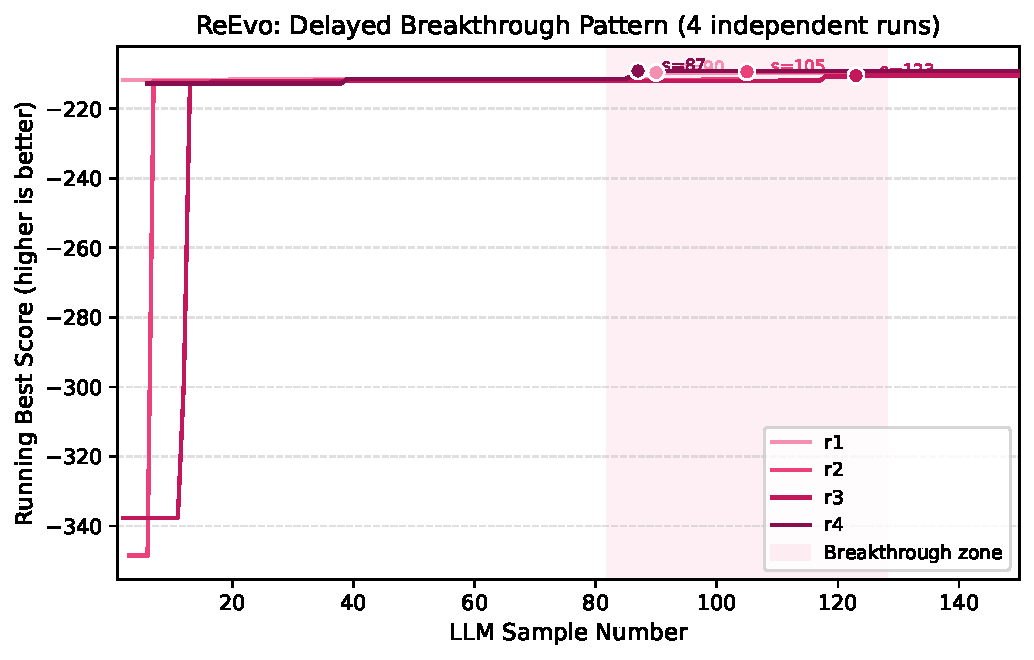
\includegraphics[width=0.65\linewidth]{reevo_breakthrough.pdf}
\caption{Per-run ReEvo convergence curves. All four runs show a late improvement
at roughly sample $87$--$123$, after an initial plateau.}
\label{fig:reevo}
\end{figure}

All four ReEvo runs (Figure~\ref{fig:reevo}) show an early plateau followed by a
late-stage improvement between samples $87$ and $123$, qualitatively consistent with
the hypothesis that the reflection buffer needs to accumulate high-scoring strategies
before it can inform the proposer. $n{=}4$ precludes a causal claim.

\section{Discussion}
\label{sec:disc}

\textbf{Dedup may subsume first-order diversity.} The $38\%$ samples-to-best
reduction together with the exploratory BCR curves ($n{=}1$ per condition) are
consistent with the hypothesis that removing behavioural redundancy already
delivers much of the exploration effect that explicit diversity mechanisms target,
and that stacking filter-level diversity on top can in fact slow cluster
visitation, spreading points within already-reached clusters rather than reaching
new ones. This would echo Novelty Search's observation that penalising redundancy
can substitute for rewarding novelty directly \citep{lehman2011novelty};
confirming it requires multi-seed replication.

\textbf{Cosine on discrete decision vectors is degenerate.} On $53$ calibration
programs, $98.5\%$ of genuinely different fingerprint pairs had cosine
similarity $>0.98$: high-dimensional integer vectors whose entries share narrow
ranges (bin indices in $[0,20]$) dilute the $1$--$2$ mismatched coordinates.
Level~2 is therefore disabled, so the fingerprint-match stage itself produces no
threshold-based false positive. This does not prove out-of-distribution
equivalence (\S\ref{sec:lim}~\#4); the practical takeaway is that discrete
measures (Hamming/edit distance) or learned metrics are prerequisites for any
high-dimensional behavioural similarity filter.

\textbf{Reflection-plus-stack consistent with landscape smoothing.} The full-stack
condition's low mean ($-209.66$) and low variance ($0.59$), together with the
late-breakthrough pattern (\S\ref{sec:breakthrough-exp}), are qualitatively
consistent with \citet{ye2024reevo}'s landscape-smoothing mechanism. Because
reflection runs with dedup and diversity both active, we cannot isolate its
contribution here; $n{=}4$ further precludes a causal claim.

\section{Related Work}
\label{sec:related}

\textbf{LLM-driven evolutionary program search.} FunSearch \citep{romera2023mathematical}
established LLM-evolve for heuristic discovery; AlphaEvolve \citep{alphaevolve2025}
scaled it to industrial tasks and identifies FunSearch's single-LLM / single-evaluator
structure as a limiting factor \citep[\S5]{alphaevolve2025}. EoH \citep{liu2024eoh}
and the online-bin-packing survey \citep{sim2025bin} explore the same space for
combinatorial heuristics. We retain FunSearch's minimalist loop and target the
proposer's sample efficiency at the behaviour level.

\textbf{Reflection and behaviour-driven search.} ReEvo \citep{ye2024reevo}
introduces LLM reflection between generations; we integrate it inside the FunSearch
loop. Novelty Search \citep{lehman2011novelty} and MAP-Elites
\citep{mouret2015illuminating} established behavioural-coverage metrics; BCR is
inspired by MAP-Elites but measures cluster visitation over time. Van
Stein et al.~\citep{vanstein2025llm} advocate behaviour-space analysis for
LLM-driven meta-heuristics via runtime trajectories; our fingerprint uses probe
decisions as a different behavioural proxy.

\textbf{Duplicate suppression and semantic equivalence.} Program-search systems
commonly deduplicate \emph{syntactically} via AST-normalised hashing (as in
FunSearch's default loop \citep{romera2023mathematical}), which misses renamings
and arithmetic rewrites. Deciding \emph{semantic} equivalence is undecidable in
general; testing-based equivalence---executing candidates on a fixed probing
suite and comparing outputs---sits between these extremes and is closely related
to output-caching of deterministic LLM calls. Our funnel instantiates this middle
ground: the $375$-dim fingerprint hashes \emph{per-item placement decisions} on a
fixed probing suite, so it detects behaviourally equivalent programs that differ
syntactically, while remaining a coarse-grained proxy rather than a full
input-output cache over the target distribution.

\section{Limitations}
\label{sec:lim}

\textbf{(1) Sandbox bypass:} probes run via \texttt{exec()} with a $5$\,s timeout;
production use should route probing through the forked sandbox.
\textbf{(2) Statistical power:} $n{=}2$--$4$ runs do not meet significance thresholds.
\textbf{(3) Filter-level only:} adaptive-$\beta$ cluster scoring
($\mathrm{Perf}+\beta\cdot\mathrm{Div}$) is future work.
\textbf{(4) Probe generalisation:} $375$-decision fingerprint equivalence is
not verified end-to-end on the full OR3 distribution (O2 is indirect evidence).
\textbf{(5) BCR/t-SNE scope:} Dedup and Dedup+Div only, $n{=}1$ per condition
(exploratory rather than a mechanism claim).
\textbf{(6) Reflection-only not ablated:} the \textit{reevo} condition runs
reflection on top of dedup and filter-level diversity, so ReEvo's contribution
cannot be isolated here; a reflection-only run (\texttt{REEVO\_ENABLED=1,
DIVERSITY\_ENABLED=0}) is deferred to follow-up work.

\section{Conclusion}
\label{sec:conc}

Behavioural-fingerprint deduplication cuts FunSearch's samples-to-best by $38\%$ on
OR3 online bin packing without degrading best score. Exploratory BCR analysis
($n{=}1$ per condition) suggests that filter-level diversity \emph{may} slow
cluster coverage, and the full stack with ReEvo gives the lowest-variance condition
in our $n{=}4$ runs, consistent with landscape smoothing. Future work:
adaptive-$\beta$ cluster scoring, a reflection-only ablation, and larger sample
budgets for significance testing.

\bibliography{final}
\bibliographystyle{iclr2024_conference}

\appendix

\section{Reproducibility and Implementation Notes}
\label{app:repro}

All results are logged from runs conducted between 2026-04-15 and 2026-04-21 on
the course-provided \texttt{gpt-5-nano} endpoint. Per-condition run seeds, log
files, and the aggregation script are included in the released repository; the
reported means and standard deviations are reproduced exactly by
\texttt{scripts/collect\_results.py}.

\textbf{API robustness.} The LLM wrapper uses a $60$\,s socket timeout and at
most $5$ exponential-backoff retries, configurable via \texttt{API\_TIMEOUT}
and \texttt{API\_MAX\_RETRIES} environment variables. This bound was added on
2026-04-21 to cap wall-clock on re-runs; it does not affect the logged
$150$-sample results, which completed under a previous, unbounded retry
configuration. The Colab notebook linked in the abstract regenerates every
table and figure from the raw CSV logs without rerunning the LLM loop.

\section{Probing Instances}
\label{app:probes}

\begin{table}[H]
\centering\small
\begin{tabular}{@{}lrrl@{}}
\toprule
Name & Capacity & Items & Description \\
\midrule
or3\_sample        & 150 & 40 & First 40 items of OR3 \texttt{u500\_00} \\
medium\_uniform    & 150 & 40 & $[30,31,\dots,69]$; pairwise packing possible \\
large\_items       & 150 & 35 & $[75,76,\dots,109]$; $\le 2$ per bin \\
small\_varied      & 150 & 40 & Non-monotonic items in $[20,38]$ \\
bimodal            & 150 & 36 & $18$ large ($\sim 100$) + $18$ small ($\sim 25$) \\
descending\_spread & 150 & 35 & $140,137,\dots,38$ (FFD-style stress) \\
ascending\_spread  & 150 & 35 & $25,28,\dots,127$ \\
sawtooth           & 150 & 36 & Periodic $\{30,50,70,90,110,130\}\times 6$ \\
tight\_pairs       & 100 & 40 & Items $\sim 50\%$ capacity; many feasible bins \\
wide\_capacity     & 200 & 38 & Deep bin states, items in $[30,100]$ \\
\midrule
Total              &     & 375 & Fingerprint dimensionality \\
\bottomrule
\end{tabular}
\caption{Ten probing instances used to compute behavioural fingerprints. Each
instance is deterministic; the fingerprint is the concatenation of the online
bin-assignment decisions over all $375$ items.}
\label{tab:probes}
\end{table}

\section{ReEvo Reflection Prompt}
\label{app:reevo}

After a candidate program is accepted (passes dedup and receives a valid score), we
issue the following reflection call to the same LLM backbone:

\begin{quote}\small
\texttt{The following Python function is a heuristic for online bin packing. It scored
\{score\} (higher is better; optimal is around $-200$).}\\[0.5ex]
\texttt{```python\\
\{program body\}\\
```}\\[0.5ex]
\texttt{In $1$--$2$ sentences, describe the algorithmic strategy this function uses and
how it differs from a simple greedy approach. Be concise.}
\end{quote}

The reflection text (max $150$ tokens) is stored by program-body hash. At prompt
construction time, the top-$3$ reflections by score are appended as
Python comments under the header \texttt{\# Strategy insights from top-performing
programs:} before the next LLM call.

\section{Hyperparameters}
\label{app:hparams}

\begin{table}[h]
\centering\small
\begin{tabular}{@{}lll@{}}
\toprule
Component & Parameter & Value \\
\midrule
FunSearch  & \texttt{num\_islands}            & $10$ \\
           & \texttt{samples\_per\_prompt}    & $4$ \\
           & \texttt{functions\_per\_prompt}  & $2$ \\
           & \texttt{cluster\_sampling\_temperature\_init} & $0.1$ \\
           & \texttt{evaluate\_timeout\_seconds} & $30$ \\
LLM        & model                            & \texttt{gpt-5-nano} \\
           & \texttt{max\_tokens}             & $4096$ (main), $150$ (reflection) \\
Dedup      & \texttt{level0\_enabled}         & \texttt{True} \\
           & \texttt{level1\_enabled}         & \texttt{True} \\
           & \texttt{level2\_enabled}         & \texttt{False} (see \S\ref{sec:fp}) \\
           & \texttt{cosine\_threshold}       & $0.98$ \\
           & \texttt{probe\_timeout\_seconds} & $5$ \\
Diversity  & \texttt{beta\_init}              & $0.3$ \\
           & \texttt{beta\_decay\_period}     & $350$ \\
ReEvo      & \texttt{max\_reflections}        & $20$ \\
           & top-$k$ for prompt               & $3$ \\
\bottomrule
\end{tabular}
\caption{Hyperparameter summary. Sources: \texttt{implementation/config.py},
\texttt{src/dedup/dedup\_config.py}, and the ReEvo integration block of
\texttt{funsearch\_bin\_packing\_llm\_api.py}.}
\label{tab:hparams}
\end{table}

\end{document}
